\section{Issues with Diffusion Models}
\begin{frame}{}
    \LARGE Diffusion Models: \textbf{Issues with Diffusion Models}
\end{frame}


% --- Issues with Diffusion Models ---
\begin{frame}{Issues with Diffusion Models}
\begin{itemize}
    \item \textbf{Slow Sampling:} Diffusion models require hundreds to thousands of iterative steps to generate a sample, making them computationally expensive and slow compared to other generative models.
\end{itemize}
\end{frame}

% --- Generative Learning Trilemma ---
\begin{frame}{Trilemma of Generative Learning}
    \begin{figure}
        \centering
        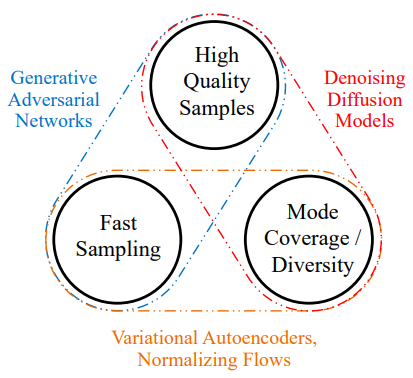
\includegraphics[height=0.8\textheight, width=\textwidth, keepaspectratio]{images/diffusion/trilemma.png}
        \caption*{Generative Learning Trilemma: Balancing sample quality, diversity, and fast sampling.}
    \end{figure}
    \footnotetext{\href{https://arxiv.org/abs/2112.07804}{Tackling the Generative Learning Trilemma with Denoising Diffusion GANs}}
\end{frame}

% --- Incremental: Current Research Directions ---
\begin{frame}[allowframebreaks]{Diffusion Models: Current Research Directions}
\begin{itemize}
    \item \textbf{Faster Sampling:}
    \begin{itemize}
        \item \href{https://arxiv.org/abs/2010.02502}{Denoising Diffusion Implicit Models (DDIM):} 
        Propose a non-Markovian process for faster and deterministic sampling by skipping steps and refining the sample.
    \end{itemize}
    \item \textbf{Improved Training:}
    \begin{itemize}
        \item \href{https://arxiv.org/abs/2102.09672}{Improved Denoising Diffusion Probabilistic Models:}
        Learn the noise variance $\sigma^2$ during training, rather than fixing it, for better flexibility and performance.
    \end{itemize}
    \item \textbf{Score-Based Modeling:}
    \begin{itemize}
        \item \href{https://arxiv.org/abs/2011.13456}{Score-Based Generative Modeling through SDEs:}
        Model the gradient of the log-density (score function) using stochastic differential equations for improved sample quality.
    \end{itemize}
\framebreak
    \item \textbf{Combining GANs and Diffusion:}
    \begin{itemize}
        \item \href{https://arxiv.org/abs/2112.07804}{Denoising Diffusion GANs:}
        Use GANs to model each denoising step, addressing the trilemma by improving speed and sample quality.
    \end{itemize}
    \item \textbf{High-Fidelity Generation:}
    \begin{itemize}
        \item \href{https://arxiv.org/abs/2106.15282}{Cascaded Diffusion Models:}
        Employ a cascade of diffusion models at different resolutions to boost sample fidelity.
    \end{itemize}
\end{itemize}
\end{frame}
